\begin{table}[h]
    \centering
    \caption{Comparação do Tempo do Insertion Sort, Merge Sort e Quick Sort}
    \begin{tabular}{|c|c|c|c|c|c|c|}
        \hline
        Tamanho de Entrada & 10 & 100 & 1000 & 10000 & 100000 & 1000000 \\
        \hline
        Insertion & 0.000000 & 0.000000 & 0.001000 & 0.103000 & 10.177000 & 1089.101000 \\
        \hline
        Merge & 0.000000 & 0.000000 & 0.000000 & 0.001000 & 0.008000 & 0.099000 \\
        \hline
        QuickV1 & 0.000000 & 0.000000 & 0.002000 & 0.139000 & 14.307000 & 1456.626000 \\
        \hline
        QuickV2 & 0.000000 & 0.000000 & 0.000000 & 0.000000 & 6.522145 & 1240.6443000 \\
        \hline
        QuickV3 & 0.000000 & 0.000000 & 0.000000 & 0.001000 & 7.0014000 & 151.0000230\\
        \hline
        QuickV4 & 0.000000 & 0.000000 & 0.000000 & 0.000000 & 0.008000 & 0.316000 \\
        
        \hline
    \end{tabular}
    \label{tab:geralx}
\end{table}

Para a elaboração da tabela (Tabela \ref{tab:geralx}) e do gráfico (Figura \ref{fig:geralx1}), foi desenvolvido um algoritmo em C com o intuito de gerar arquivos de diferentes tamanhos de entrada, 10, 100, 1.000, 10.000, 100.000 ou 1.000.000, contendo sequências de números, bem como seus n sucessores. Essas sequências puderam ser geradas em ordem Crescente, Decrescente ou Aleatória. Os resultados obtidos revelam características do funcionamento do Insertion Sort, Merge Sort e Quick Sort. 

Observando a performance desses algoritmos, notamos que o Insertion Sort, embora simples e eficiente para pequenos conjuntos de dados ou conjuntos quase ordenados, tende a ser menos eficaz em entradas maiores, onde seu desempenho se deteriora. O Merge Sort, por outro lado, mantém uma performance estável e eficaz, independentemente da configuração inicial dos dados. Ele é particularmente eficiente em ordenar grandes volumes de dados e é conhecido por sua complexidade de tempo O(n log n). 

O Quick Sort se destaca por sua velocidade média, especialmente em entradas desordenadas, graças ao seu processo de divisão e conquista. No entanto, sua performance pode variar dependendo da escolha do pivô e da configuração dos dados, o que o torna menos previsível em alguns casos. No geral, o Merge Sort e o Quick Sort são frequentemente preferidos em cenários de ordenação de grande escala, devido à sua eficiência em comparação com o Insertion Sort.



\begin{figure}[H]
    \centering
    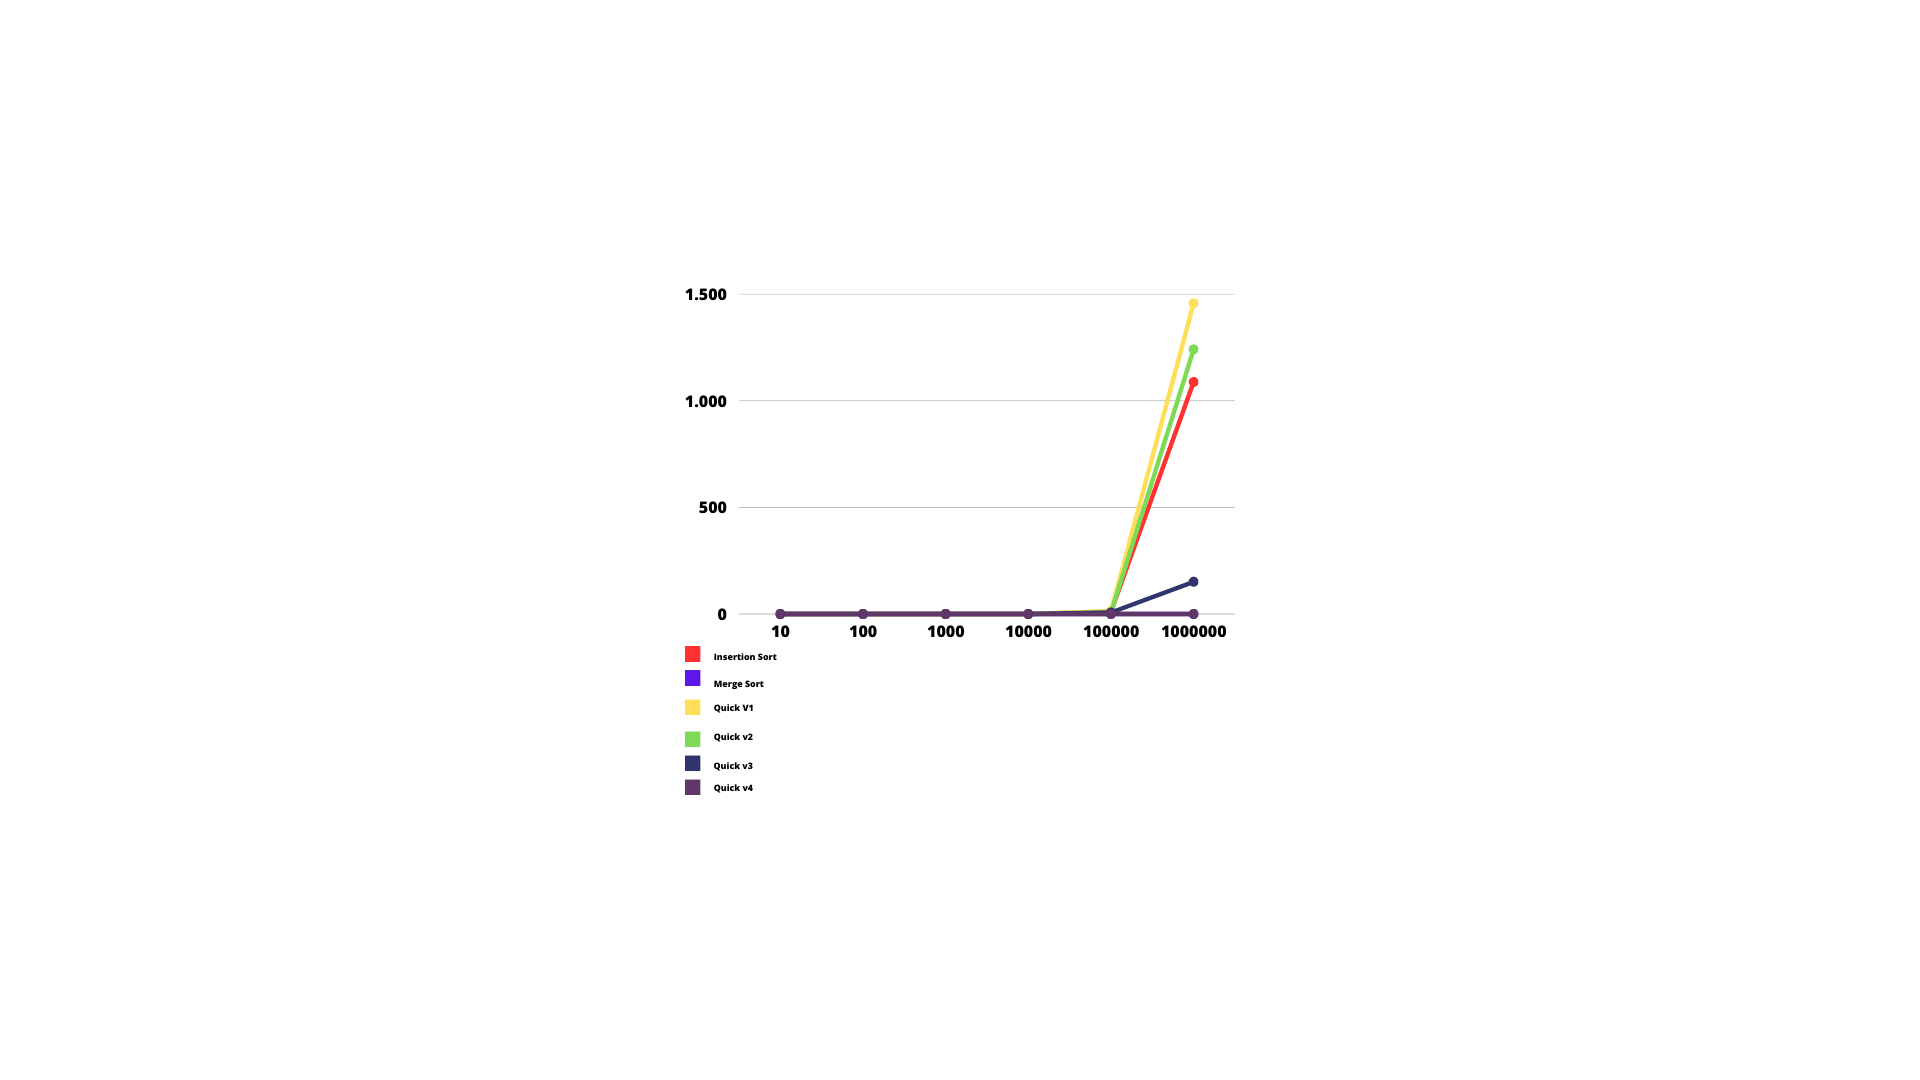
\includegraphics[width = 20cm]{Imagens/Quickx Sort/graficogeral.png}
    \caption{Gráfico de tempo do algoritmo Insertion Sort, Merge Sort e Quick Sort.}
    \label{fig:geralx1}
\end{figure}